\chapter{Introdução}
O crescimento no consumo de energia cada vez mais vem aumentando conforme os anos, segundo \cite{balanco_energetico}, o
Brasil consumiu 531.1 TWh no ano de 2014, resultando em um aumento de 2.9\% comparado à 2013.

O Brasil possui uma matriz energética predominantemente renovável tendo como ênfase a geração hidráulica, as fontes renováveis correspondem à 84.1\% e não renováveis 26.9\%, conforme ilustrado na imagem \ref{consumo-2014}.

\begin{figure}[h]
    \centering
    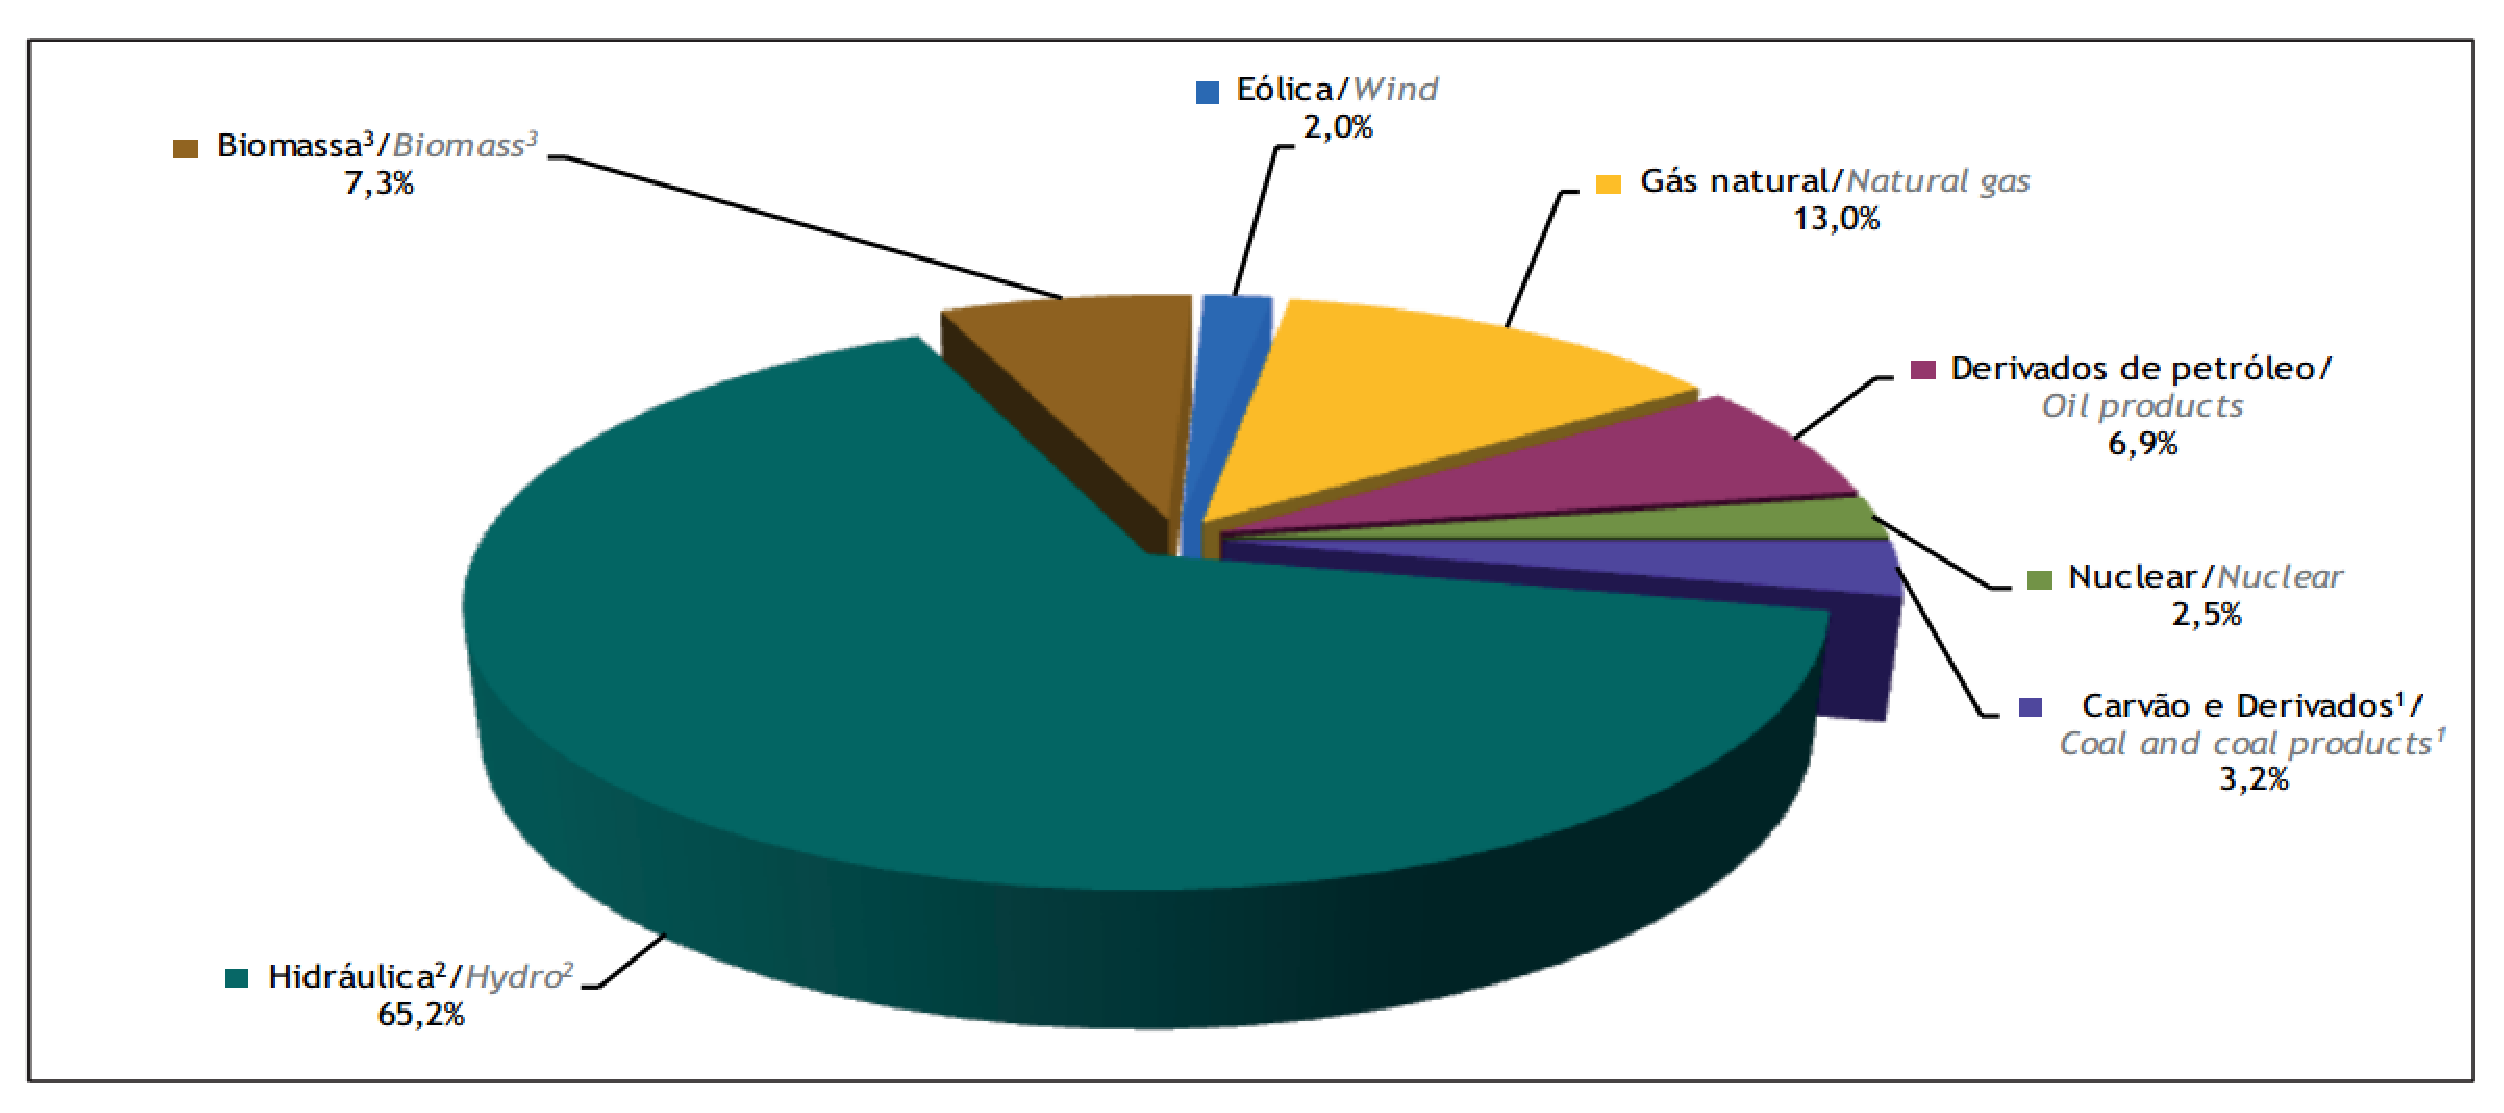
\includegraphics[keepaspectratio=true,scale=0.4]{figuras/consumo_energia_2014.eps}
    \caption{Oferta Interna de Eletricidade no Brasil em 2014}
    \label{consumo-2014}
\end{figure}

Texto sobre consumo de energia em prédios públicos.

No ano de 2015 foi realizado um reajuste tarifário da energia elétrica correspondente à 33\% para clientes residenciais e 32,5\% para empresas, indústrias e comércios
\cite{aumento_energia}, gerando altos gastos à população devido ao seu uso excessivo.

Dentre as alternativas para reduzir o consumo de energia elétrica encontram-se o uso de equipamentos mais eficientes, certificações Procel, uso racional da energia e afins, porém, quando se trata de instalações de grande porte, como Universidades e órgãos públicos em geral, percebe-se que um dos grandes problemas enfrentado é a falta de monitoramento adequado do uso de energia elétrica.

\textit{Software} entrega o mais importante produto da atualiadade: informação. Transforma informações
pessoais para que a mesma seja mais útil em um contexto local; gerencia informações de negócio para
melhorar a competitividade; Fornece uma porta de acesso a redes de informação em todo o mundo (por
meio da \textit{Internet}) e fornece os meios para adquirir informação em todas as suas formas (\cite{pressman_2009}).

Os negócios atualmente operam em um ambiente global sujeito a rápidas mudanças sendo crucial
estar preparado para novas oportunidades de mercado, mudanças de condições econômicas e ao surgimento
de produtos e serviços concorrentes. O \textit{software} é um dos componentes cruciais para a realização
de todas as operações de negócio e realizá-lo de forma rápida também é uma maneira de aproveitar novas
oportunidades e responder às pressões competitivas \cite{sommerville_2006}.

Em Janeiro de 2016, a Prefeitura de Campus da Universidade de Brasília realizou a aprovação de um projeto que
idealiza um sistema capaz de realizar o gerenciamento energético da própria Universidade.

\section{Objetivo Geral}
Desenvolver sistema web capaz de monitorar, em tempo real, medições de energia coletadas por transdutores
instalados em quadros de energia da Universidade de Brasília.

\subsection{Objetivos Específicos}
O sistema deve ser capaz de:
\begin{itemize}
    \item Cadastrar/Editar/Remover transdutores.
    \item Utilizar rede da universidade para comunicar-se com transdutores.
    \item Realizar a coleta de dados de forma automatizada e temporizada.
    \item Mostrar aos usuários os dados de energia coletados.
\end{itemize}

\section{Metodologia Utilizada}
A metodologia abordada neste trabalho teve como base o desenvolvimento de um \textit{software} livre
utilizando-se dos princípios empíricos de desenvolvimento ágil de \textit{software} juntamente com práticas do Scrum e \textit{Extreme Programming}.

\section{Estruturação do Trabalho}
O trabalho encontra-se estruturado da seguinte maneira:

\begin{itemize}
    \item Capítulo 2: abordará os métodos empíricos em engenharia de \textit{software} utilizados para
    auxiliar no desenvolvimento do sistema.
    \item Capítulo 3: abordará como estruturou-se a gerência de configuração.
    \item Capítulo 4: abordará as princípais tecnologias \textit{web} e protocolos de comunicação utilizados.
    \item Capítulo 5: abordará a evolução do desenvolvimento do sistema relatando o que foi realizado durante cada \textit{sprint}.
    \item Capitulo 6: abordará uma conclusão preliminar sobre o que foi/resta a ser desenvolvido.
\end{itemize}